\documentclass{article}
\usepackage{titlesec}
\usepackage{graphicx}
\graphicspath{images/}
\usepackage{wrapfig}

\usepackage{blindtext} %This is for placeholder text

\usepackage{hyperref}

%Setting up the style of hyperlinks and URLs in the document

\hypersetup{
    colorlinks=true,
    linkcolor=blue,
    filecolor=magenta,      
    urlcolor=cyan
    }

\urlstyle{same}

%Document attribution and title

\title{Debian Configuration Automation}
\author{Ryan Piazza}

%Actual document contents

\begin{document}

\tableofcontents

\maketitle


\section{Introduction}

The rationale for using this is to easily get Debian systems up and running, repeatedly. I have personally gone through the graphical installer tens (if not hundreds) of times. Because of this, I feel the need to get a basic script going that can replicate my settings on a repeated basis. 

I've blown up enough systems trying to install some tweak and then not been able to figure out how to get it back. Hopefully, this can help. 

\section{What it Does}

The script automates the installation of packages, configs, DEs, etc. This is after the initial installation. 

\blindtext





\section{Installing Debian}

Most of this section is just a formality for the sake of covering all bases, but it can be a helpful refresher for anybody who hasn't done it in a while or a quick tutorial if you've never done it at all. 

Installing Debian requires a disc image, an ISO\footnote{"ISO" comes from the ISO 9660 file system standard for CD-ROMs}. The ISO for Debian can be found on their website, which is located \href{https://www.debian.org/distrib/}{here}. There are many different versions of Debian you can choose from. 

Debian distributions are broken down into three types:
\begin{enumerate}
    \item Stable - codenamed "trixie"
    \item Testing - codenamed "forky"
    \item Unstable - codenamed "sid"
\end{enumerate}

In most cases, Debian is considered stable due to separating out bleeding edge features from the main distribution (i.e., Stable). This is as opposed to a rolling release distro, like Arch, which is more prone to breaking but will provide the desktop user with the newest possible developments\footnote{For this reason, Debian is often used as an OS for servers.}. 

After downloading the ISO, you can decide whether to virtualize or run the OS on bare metal (hardware). There are advantages and disadvantages to both, the details of which can be found elsewhere\footnote{See Professor Messer on YouTube for some great information}.

\subsection{On Bare Metal}

\begin{wrapfigure}{1}{.35\textwidth}
    \centering 
    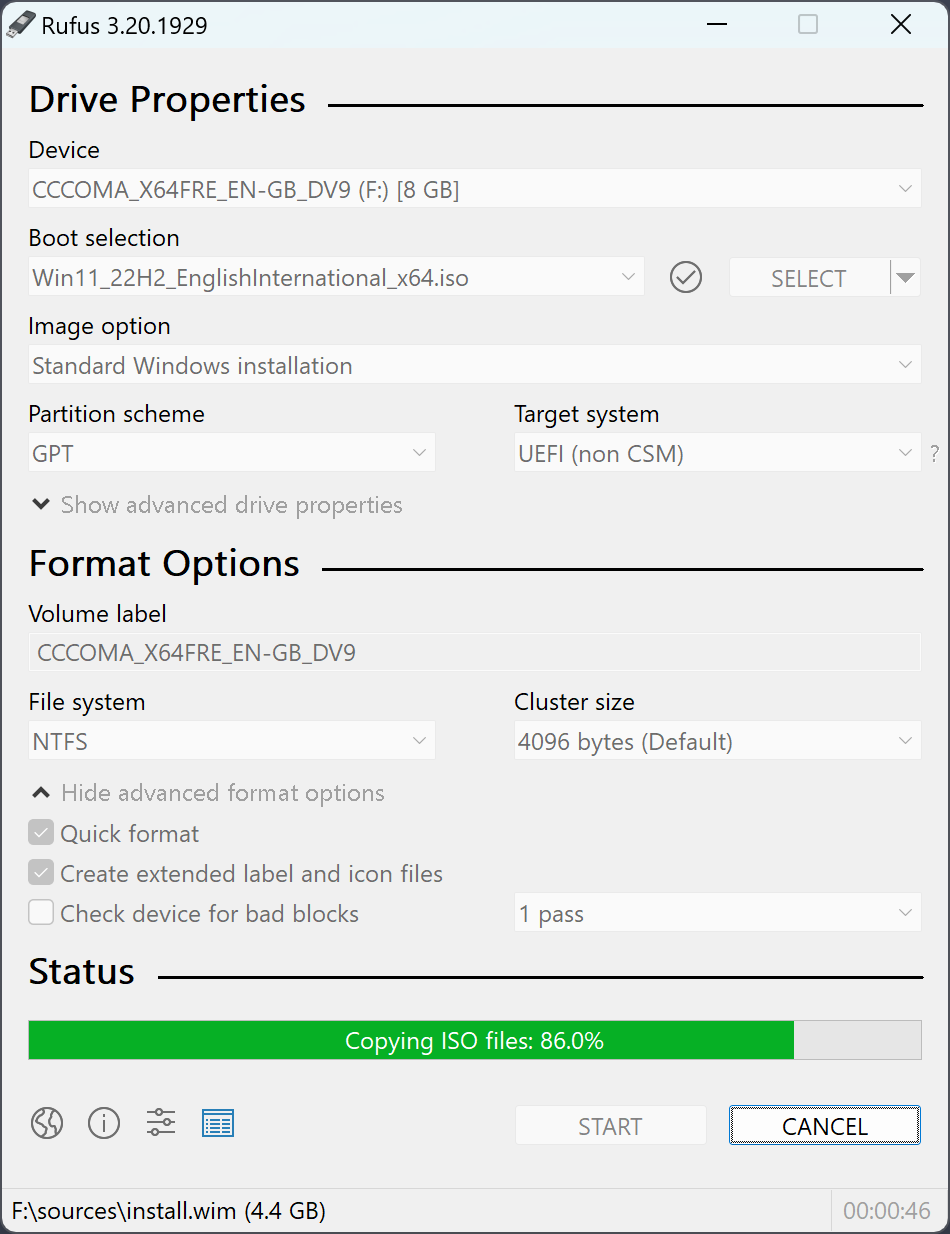
\includegraphics[width=.35\textwidth]{images/rufus.png}
\end{wrapfigure}

Bare metal installation requires creating bootable media, which means using some software that can get a USB stick ready. For Windows users, I recommend the Rufus program which you can find \href{https://rufus.ie/en/}{here}. 

Select the device from the top dropdown (the USB stick), select the Debian ISO in the boot selection area. Partition scheme and target system will be determined by your PC, but this can mostly be eschewed if you select GPT as the Partition scheme and UEFI (non CSM) as the Target system. Ensure that this will work in the BIOS system setup. 

After Rufus creates the device, boot into it by rebooting the desired PC and selecting the USB stick in the BIOS system setup boot menu.

After this, Debian will guide you through a graphical installation process. 

\subsection{In a Virtual Machine}

Installing on a VM is much easier. No bootable instllation media is required. Instead, select the ISO in whatever your chosen platform's virtual disk drive manifests as, then move it to the top of the boot order. 

This should boot you into the Debian grphical installation menus. 

\section{Script Setup}

\blindtext

\section{Support}

\blindtext

\section{Licensing}

  Copyright \textsuperscript{\textcopyright} 2025 Ryan Piazza

    This program is free software: you can redistribute it and/or modify
    it under the terms of the GNU General Public License as published by
    the Free Software Foundation, either version 3 of the License, or
    (at your option) any later version.

    This program is distributed in the hope that it will be useful,
    but WITHOUT ANY WARRANTY; without even the implied warranty of
    MERCHANTABILITY or FITNESS FOR A PARTICULAR PURPOSE.  See the
    GNU General Public License for more details.

    You should have received a copy of the GNU General Public License
    along with this program.  If not, see \href{https://www.gnu.org/licenses/}{https://www.gnu.org/licenses/}.

\end{document}
